\chapter{Validación}
En este capítulo se muestran dos formas de validación para este trabajo. La primera, muestra la experiencia de programar una pequeña aplicación Dart con facetas públicas. La segunda, muestra los tests unitarios utilizados para comprobar las reglas del sistema de tipos de la desclasificación basada en tipos.


\section{Programando con facetas públicas}
Para ilustrar la interacción entre el programador, el sistema de inferencia y la extensión para ambientes de desarrollo, se mostrará paso a paso la creación de una pequeña aplicación de \emph{login} web.

Primero, se crea la clase \texttt{Database} que simula una base de datos de usuarios registrados, mediante una estructura \texttt{Map}.
\vspace{0.5em}
\begin{lstlisting}
  class Database {
    Map<String, int> get data => {
      "mmeneses@dcc.uchile.cl": "12345".hashCode,
      "matias.imc@gmail.com": "123456".hashCode,
    };
  }
\end{lstlisting}

Luego, se crea la clase \texttt{Login} con un método \texttt{login} similar al visto en los ejemplos de los primeros capítulos.
\vspace{0.5em}
\begin{lstlisting}
  class Login {
    Database db = new Database();




    bool login(String username, String guess) {
      if (db.data.containsKey(username)) {
        if (db.data[username] == guess.hashCode) return true;
      }
      return false;
    }
  }
\end{lstlisting}

Notar que no se ha agregado ninguna faceta pública. La figura \ref{screen1} muestra la ventana del ambiente de desarrollo hasta este paso, donde se muestran las facetas públicas inferidas para todos los identificadores en la parte inferior, y una faceta pública inferida específica al ubicar el cursor sobre un identificador.

\begin{figure}[ht]
  \centering
  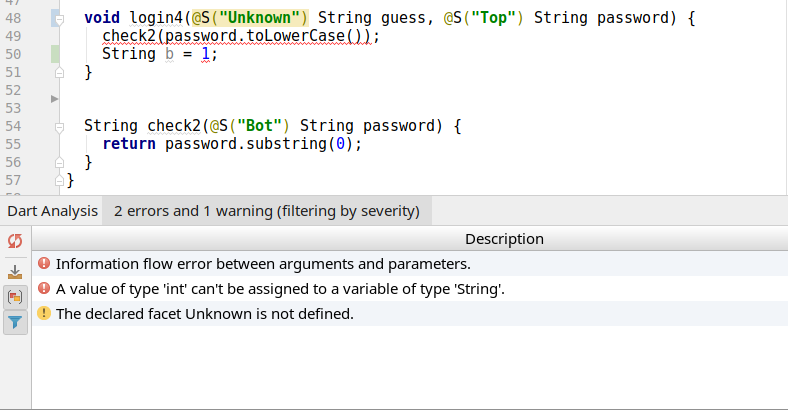
\includegraphics[width=0.7\textwidth]{imagenes/screen1.png}
  \caption{Información de la faceta pública inferida}
  \label{screen1}
\end{figure}

Ahora, se intenta agregar la faceta pública \texttt{@("Hash")} al parámetro \texttt{guess} del método \texttt{login}. Como esta faceta pública no ha sido definida, la extensión lanza un warning. La figura \ref{screen2} ilustra esta situación. Para una mejor legibilidad, se filtraron los errores mostrados en la parte inferior para que no muestre errores informativos.
\clearpage
\begin{figure}[ht]
  \centering
  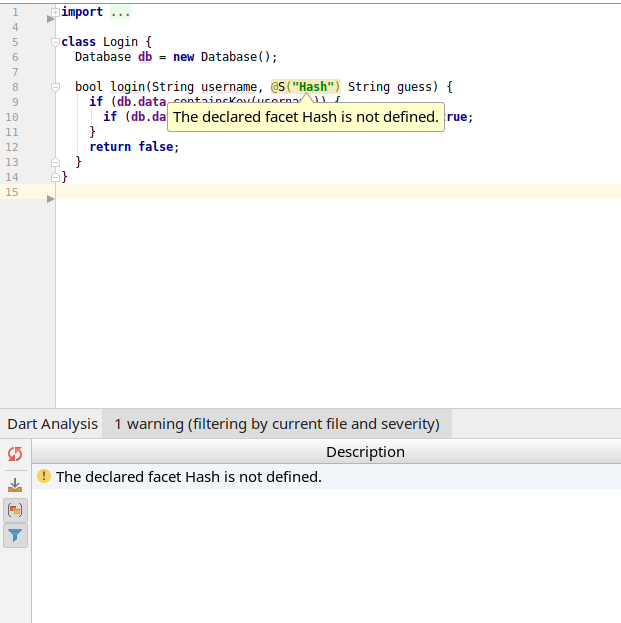
\includegraphics[width=0.7\textwidth]{imagenes/screen2.png}
  \caption{Warning por faceta pública no definida}
  \label{screen2}
\end{figure}

Entonces, se define la faceta pública \texttt{Hash} mediante una clase abstracta de Dart. Además, se definen algunas facetas públicas adicionales para la clase \texttt{Database}, debido a que el flujo de información desde la base de datos debe ser controlado.
\vspace{0.5em}
\begin{lstlisting}
  abstract class Hash {
    int get hashCode;
  }
  abstract class Data {
    int get data;
  }
  abstract class ContainsKeyAndGetHash {
    bool containsKey(Object key);
    @S("Top") bool operator [](Object key);
  }
  class Database {
    @S("Data") Database();

    @S("ContainsKeyAndGetHash") Map<String, int> get data => {
      "mmeneses@dcc.uchile.cl": "12345".hashCode,
      "matias.imc@gmail.com": "123456".hashCode,
    };
  }
  class Login {
    Database db = new Database();

    bool login(String username, @S("Hash") String guess) {
      if (db.data.containsKey(username)) {
        if (db.data[username] == guess.hashCode) return true;
      }
      return false;
    }
  }
\end{lstlisting}

Ahora, se crea la clase \texttt{Home} que se encarga de renderizar la página, utilizando la librería html de Dart. Notar que esta clase obtiene un valor desde un campo de contraseña. La variable \texttt{guess} que es asignada con ese valor declara una faceta pública \texttt{Top}. Luego se intenta realizar la autenticación con el método \texttt{login}.
\vspace{0.5em}
\begin{lstlisting}
  class Home {
    void render() {
      Login login = new Login();
      querySelector('#button').onClick.listen((MouseEvent e) {
        InputElement emailField = querySelector('#email');
        InputElement passwordField = querySelector('#password');
        String username = emailField.value;
        @S("Top") String guess = passwordField.value;
        if (login.login(username, guess)) {
          querySelector('#title').text = "Welcome";
        }
        else {
          querySelector('#title').text = "Bad credentials";
        }
      });
    }
  }
\end{lstlisting}

Sin embargo, la extensión reporta un error de seguridad en la invocación al método \texttt{login}. Esto ocurre porque el parámetro \texttt{guess} del método \texttt{login} declara una faceta pública \texttt{Hash}, y le estamos pasando como argumento un valor con faceta pública \texttt{Top}, lo cual es un flujo inválido. La figura \ref{screen3} muestra la ocurrencia de este error.
\clearpage
\begin{figure}[ht]
  \centering
  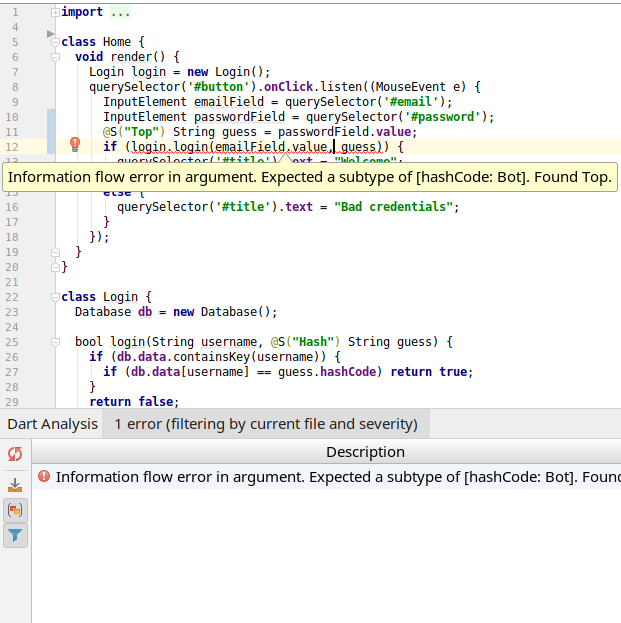
\includegraphics[width=0.7\textwidth]{imagenes/screen3.png}
  \caption{Error de seguridad}
  \label{screen3}
\end{figure}

Para solucionarlo, se asigna la faceta pública \texttt{Hash} a la variable \texttt{guess}.
\vspace{0.5em}
\begin{lstlisting}
  @S("Hash") String guess = passwordField.value;
\end{lstlisting}

 Luego, se crea el archivo \texttt{html} de la aplicación. El resultado se puede ver en la figura \ref{screen4}.

Para que la aplicación de Dart sea compatible con los navegadores, se debe realizar una compilación al lenguaje Javascript. Esta compilación genera un archivo \texttt{.js} que es posible referenciar en el archivo \texttt{html}.
\clearpage
 \begin{figure}[ht]
   \centering
   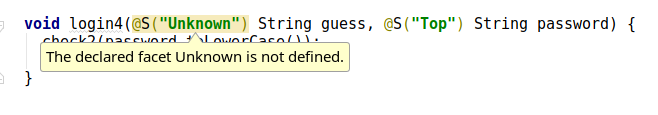
\includegraphics[width=0.5\textwidth]{imagenes/screen4.png}
   \caption{Pantalla de login}
   \label{screen4}
 \end{figure}


 En este ejemplo fue posible constatar la utilidad del sistema de inferencia. De las 22 declaraciones de identificadores del código, solo 7 de ellas fueron anotadas con facetas públicas, y el resto fue inferido de acuerdo a las reglas del sistema de tipos. Además, este ejemplo sirvió para aplicar la programación con facetas públicas en una aplicación realista. El código de la aplicación se encuentra en un repositorio de GitHub~\cite{repotest}.

\section{Batería de tests}
En conjunto con Raimil Cruz, uno de los autores del trabajo de la desclasificación basada en tipos, se validaron una serie de tests unitarios que ponen a prueba el cumplimiento de las reglas del sistema de tipos. Estos tests se encuentran en el repositorio de GitHub de la herramienta~\cite{repounit}.

Además de proveer una forma de validación de este trabajo, los tests unitarios sirvieron como guía para la implementación de las distintas componentes.

Para escribir los tests se utilizó la librería estándar de testing en Dart.

\section*{Resumen}
En este capítulo se mostró el proceso de programar una aplicación realista con facetas públicas, mostrando la interacción entre el usuario y la herramienta. En el siguiente capítulo se presentan las conclusiones de la memoria y el trabajo futuro.
